\documentclass[../../Main/Appunti Fisica.tex]{subfiles}
\begin{document}
Si consideri la figura di seguito riportata.
\begin{figure}[!h]
    \centering
    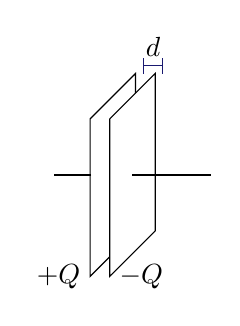
\begin{tikzpicture}[scale = 1, every node/.style={scale=1}]

        % Condenser plates
        \filldraw [fill = white] (0.75, -0.25, -1.5) -- (0.75, 0, -1.5) -- (0.75, 0, 0) -- (0.75, -2, 0) -- (0.75, -2, -0.75);
        \filldraw [fill = white] (1, 0, 0) -- (1, 0, -1.5) -- (1, -2, -1.5) -- (1, -2, 0) -- (1, 0, 0);

        \node [anchor = east] at (0.75, -2, 0) {\(+ Q\)};
        \node [anchor = west] at (1, -2, 0) {\(- Q\)};

        % Condenser cables
        \draw (1, -1, -0.75) -- (2, -1, -0.75);
        \draw (0.475, -1, -0.75) -- (0, -1, -0.75);

        \draw [|-|, color = MidnightBlue] (0.75, 0, -1.75) -- (1, 0, -1.75);
        \node [anchor = south] at (0.875, 0, -1.75) {\(d\)};
    \end{tikzpicture}
    \caption{Schema di condensatore a facce piane.}
    \label{fig:13}
\end{figure}

Se si trascurano gli effetti lungo i bordi, se la distanza \(d\) tra le piastre è piccola, segue
\[
    \va{E} = \frac{\sigma}{\varepsilon_{0}} = \frac{Q}{\varepsilon_{0} A}
\]
%
Poiché il campo tra le armature è uniforme, \(\Delta V = \vb{E} d = Q d / \varepsilon_{0} A\), da cui sostituendo all'Equazione \eqref{eq:17} segue
\[\begin{aligned}
    C = \frac{Q}{\Delta V} &= \frac{Q}{Q d / \varepsilon_{0} A} \\
    &= \frac{\varepsilon_{0} A}{d}
\end{aligned}\]
\end{document}